\section{ARC Synthesis}
Operators require support for a diverse collection of policies, 
like service chaining, traffic engineering, and isolation. Also,
since failure is handled in a distributed manner, operators need 
support for policies which specify resilience properties and behavior
of traffic under failure scenarios. 
Earlier 
work in this area has focused on finding ideal OSPF weights for 
traffic engineering~\cite{te-ospf}, but such approaches are 
inherently tied with the policies supported, and are not extensible 
to other policies easily. 

Our preliminary approach to this problem was
to specify policies using SMT theories like propositional logic and 
linear rational arithmetic and use off-the-shelf SMT solvers~\cite{z3} 
to synthesize the ARC. However, current SMT solvers are incapable of 
scaling to even small-sized topologies and number of policies, majorly
due to the fact the paths in the network are based on the weights in a 
complicated manner (shortest-path) which increases the complexity of the
encoding in SMT. Synthesizing resilient control planes with this 
approach is intractable with current state-of-art SMT solvers.

As a first step towards ARC synthesis, 
we use a network data plane (set of forwarding paths)
enforcing the operator-specified policies 
as input for synthesizing the ARC. The  
advantage of using network data planes as 
input is the ease of developing
different network management applications 
enforcing proactive policies\footnote{
Traditional control planes cannot support reactive policies, however
middleboxes can overcome this limitation.} 
as if operating over a software-defined
network, agnostic of the actual network protocols used in the network. 
Many existing network management systems like Merlin~\cite{merlin} 
and SIMPLE~\cite{simple}\footnote{
Traditional control planes cannot support 
paths with loops for service chaining cannot} developed for SDNs could be seamlessly
integrated to the architecture with minimal changes.  

For a given network data plane, the synthesis of the ARC reduces to a
variation of the {\em inverse shortest path} problem, a relatively 
unexplored algorithmic problem. 
Given an input set of paths in a directed graph, the inverse shortest path problem 
informally, is the problem of finding an assignment of weights to edges 
such that each input path is the shortest weighted path between those endpoints in 
the graph. We attempt to tackle synthesis of ARCs by formulating a set of linear
equations  equipped with an unsatisfiable core learning approach. 

While the ARC synthesis from data planes can enforce 
policies by the distributed control plane, it does not
encapsulate resilience properties of the control plane. 
To accomodate resilience properties in the ARC synthesis,
we envision two different mechanisms: concrete
backup paths and path-level policies under failure scenarios. 
We discuss this in \secref{sec:resilience}. \kausik{Could expand more,
write after resilience section is complete}

\subsection{Pure ARC Synthesis}
We first describe the synthesis of {\em pure} ARCs, i.e., 
ARC with only weighted edges and no other mechanisms like route-filters.
A pure ARC is an ideal control plane because it is able to
enforce the data plane with carefully engineered edge weights
and does not disable any link in the network (e.g., route filters
(\secref{sec:routefilter})), thus providing maximal resilience. 
% Provide insight about route-filters before.

The inputs to the synthesis algorithm are:

(1) Network Data Plane:
Since most legacy routing protocols are destination-based,
from an input data plane, we extract the forwarding
DAG (directed acyclic graph) for each destination
as the sink. The DAG will be a directed tree with the
destination as root if the multi-path
functionality is not used. We define $\Omega$ for the 
set of destinations, and $\Delta$ for  
the set of destination DAGs. 
% Write something about changes to the network manager

(2) Network Topology: 
We define the physical network topology $T = (S, L)$
as a directed graph where $S$: set of switches, and 
$L$: set of directional links. 

The output of the synthesis algorithm is a 
pure ARC with positive weights on the directional links,
such that the set of forwarding DAGs $\Delta$ are the 
shortest paths in the ARC. We define $E(sw_1, sw_2)$ as
the edge weight variable for link $sw_1 \rightarrow sw_2$. 
We generate a set of linear equations to obtain edge weights,
which are provided to a LP-solver without any optimization
objectives. 

\subsubsection{Linear Equations} \label{sec:linearequations}
We construct an directed overlay graph
by combining all the individual destination DAGs in $\Delta$.
We can disable all switches and links not in the overlay. 
These links can have arbitary large weights as they do not
feature in the shortest path for any destination. 
Given $\Omega$ and $\Delta$, we generate a set of linear equations
to find the requisite edge weights. For a path connecting two switches 
$s \rightarrow^+ t$ in a DAG, 
to enforce that the path will be the shortest, we need equations
which ensure the sum of edge weights of the path is strictly smaller than
the weight of all other paths from $s$ to $t$. However, this can incur
an exponential blowup in number of equations. Instead, we use distances 
to reduce the number of equations to a polynomial order. 

\minisection{Distance Equations}
We define $D(s,t)$ to be the distance variable from $s$ to $t$
which denotes the absolute shortest distance from $s$ to $t$. 
Trivially, $D(s,s) = 0$. For a path $s \rightarrow^+ t$ ($len \geq 1$),
the shortest distance from $s$ to $t$ is the smallest of the distances
of the paths traversed through the neighbours of $s$ to $t$. Therefore, the
following set of equations enforce the semantics of distances; 
here $s \rightarrow sw$ denotes that $sw$ is a neighbour
of $s$, and $sw \rightarrow^* t$ denotes that the path from $sw$ to $t$ contains
zero or more edges.
\begin{multline} \label{eq:dist}
\forall s, t, sw. (s \rightarrow sw \rightarrow^* t).\\
D(s, t) \leq E(s, sw) + D(sw, t)
\end{multline}
These equations ensure that $D(s,t)$ is not greater than 
the actual shortest distance from $s$ to $t$.

\minisection{Destination DAG Equations}
For each destination DAG, we add equations to ensure the 
edge weights are set such that a shortest-path forwarding in the ARC will 
follow the same paths as specified in the DAG. We use the following
property: If a path is the shortest 
path, then every subpath of the path has to be the shortest path.
\begin{figure}[h!] 
	\centering
	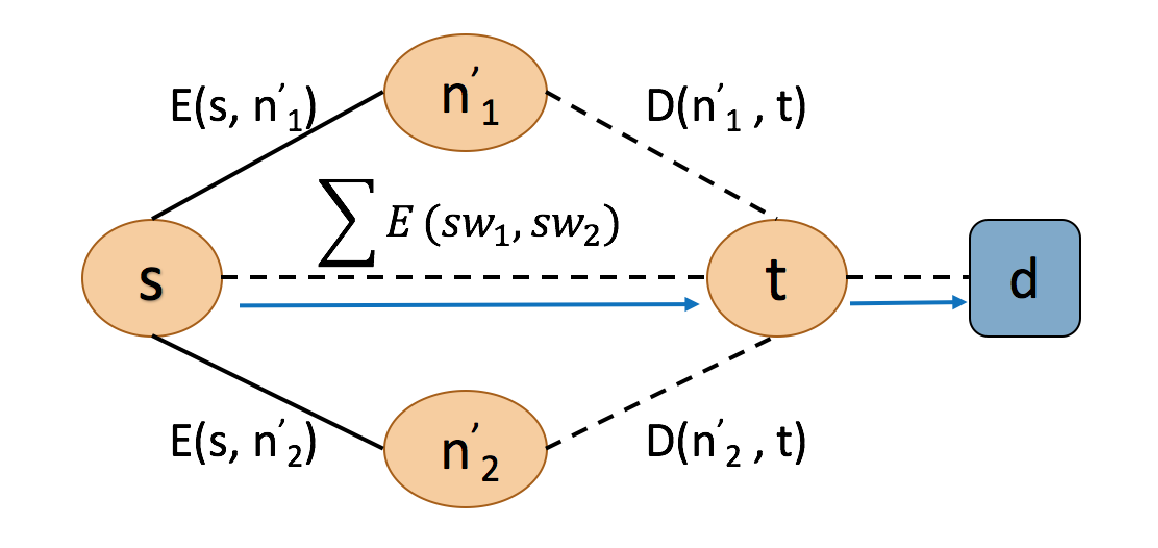
\includegraphics[width=0.8\columnwidth]{figures/distanceEquation.eps}
	\caption{Distance equation} \label{fig:disteq}
\end{figure}
Consider a DAG $\xi_d$ for destination $d$. We define two neighbour
functions: $N(s)$ denotes the neighbours of switch $s$ 
in the directed overlay graph, and $N(s, \xi_d)$ denotes
the neighbours of switch $s$ in the destination DAG. 
Since, each subpath of $\xi_d$ is the shortest path,
we need to ensure that all other
paths are not shorter or equal to these paths.  
Strict inequality is required because routing protocols
can load-balance or choose one of the equal weights paths at
random, both of which violate the DAG requirements. The weight
of a path in the DAG can be expressed as the sum of weights of 
edges along the path. 
Thus, we add the following equations to ensure the
shortest path property (\Cref{fig:disteq} illustrates 
an example).
\begin{multline} \label{eq:uniq}
		\forall d \in \Omega. \forall s, t \in \xi_d. (s \rightarrow^+ t).\\ 
		\forall n'. (n' \in N(s) \wedge n' \not\in N(s, \xi_d)). \\
		\sum_{\mathclap{\substack{(sw_1, sw_2) \in (s \rightarrow^+ t)}}} 
		E(sw_1, sw_2) < E(s, n') + D(n', t)
\end{multline}
If the path $n' \rightarrow^* t$ 
is not in any DAG completely, then
$D(n',t)$ can be smaller than the actual shortest distance by the
semantics of \Cref{eq:dist} (as
$D(n',t)$ is not equal to any quantity by \Cref{eq:shortest}).
However, since $D(n',t)$ is on the RHS of the equations in \Cref{eq:uniq},
the equations will ensure that the path $s\rightarrow n \rightarrow^* t$
has strictly greater weight than the path of the DAG.

%TODO: Add some figures